\section{Resultados}
Os resultados da execução de cada função mostra como o está o funcionamento do sua funcionalidades. 



\subsection{Amostra das execuções}



\subsubsection{Ataque de desautenticação}
O ataque demonstrou ser eficaz em provocar a desassociação do cliente do ponto de acesso. O tempo de reação do dispositivo alvo fica entre 10 e 30 segundos.
\begin{figure}[h]
    \centering
    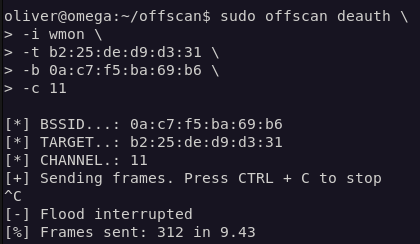
\includegraphics[width=0.45\textwidth]{fotos/deauth.png}
    \caption{Execução do mapeador de rede}
\end{figure}



\subsubsection{Descoberta de dispositivos}
No exemplo abaixo, apenas o comando para descobrir dispositivos na rede foi informado. Com isso, a interface padrão é usada e a partir do IP e da mascara da rede, todos os IPs da rede são calculados para serem escaneados.
\begin{figure}[h]
    \centering
    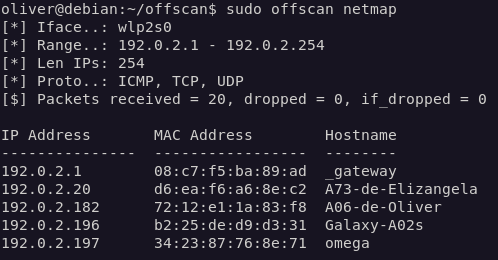
\includegraphics[width=0.46\textwidth]{fotos/hostdisc.png}
    \caption{Execução do mapeador de rede}
\end{figure}



\subsubsection{Informações de Rede e Interface}
No exemplo abaixo o comando \texttt{info} foi executado. Ele mostra informações da interface que foi escolhida e da rede ao qual está conectada, se estiver.
\begin{figure}[h]
    \centering
    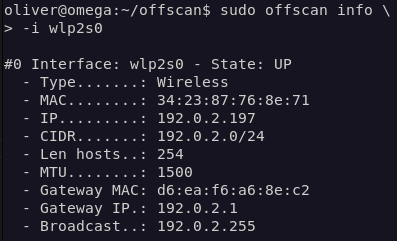
\includegraphics[width=0.46\textwidth]{fotos/info.png}
    \caption{Execução do comando \texttt{info}}
\end{figure}



\subsubsection{Mapeador de redes Wi-Fi}
No exemplo desse comando foram alterados o nome da rede (SSID) e parte do BSSID de cada rede para preservar a privacidade. A imagem abaixo mostra como o comando mostra as informações que pegou de cada rede Wi-Fi.
\begin{figure}[h]
    \centering
    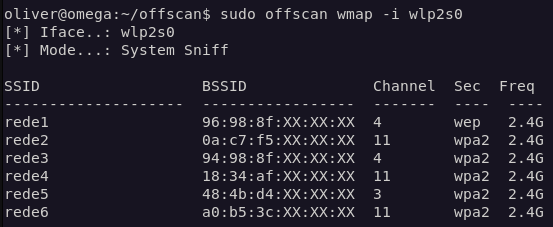
\includegraphics[width=0.46\textwidth]{fotos/wmap.png}
    \caption{Execução do mapeador de redes Wi-Fi}
\end{figure}



\subsubsection{Flooder de beacons}
O flooder de beacons se mostrou muito eficiente como mostra a imagem abaixo. Nela, é possível ver algumas das muitas redes inexistentes que os beacons transmitiram.
\begin{figure}[h]
    \centering
    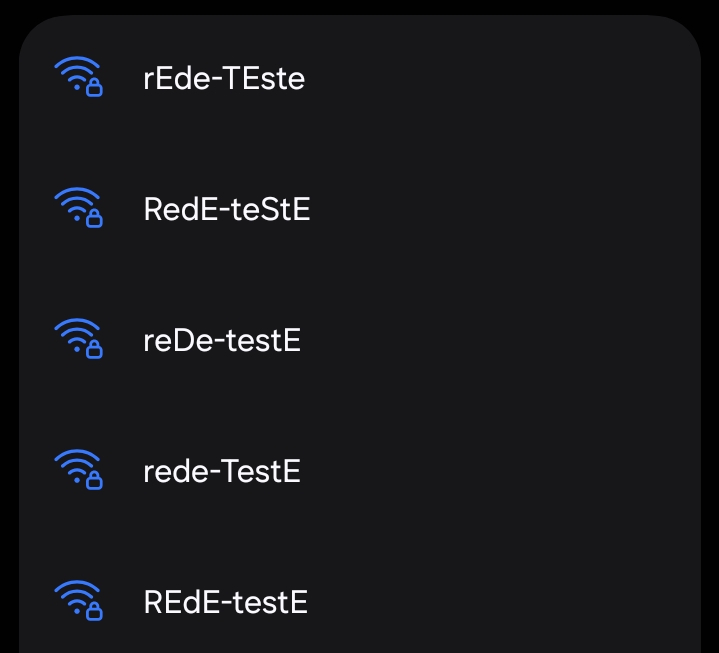
\includegraphics[width=0.46\textwidth]{fotos/beacon.jpg}
    \caption{Execução do flooder de beacons}
\end{figure}



\subsection{Análise dos resultados}
Com base nas execuções, observou-se que: 

\begin{itemize}
    \item \textbf{Flooder de beacons}: A taxa de envio foi limitada intencionalmente para evitar a saturação do espectro e permitir a visualização clara das redes falsas. Apesar dessa limitação, a funcionalidade mostrou-se eficaz, com múltiplos dispositivos detectando as redes falsas criadas.
    
    \item \textbf{Ataque de desautenticação}: O tempo médio para desconexão dos dispositivos-alvo variou entre 10 e 30 segundos. Deixando ele ativo, a reassociação automatica do dispositivo não pode ser feita. Mantendo o dispositivo sem acesso a rede.

    \item \textbf{Mapeamento Wi-Fi}: A ferramenta obteve sucesso em detectar todas as redes sem fio dentro do alcance do dispositivo. Sendo capaz de descobrir até mesmo redes ocultas.
    
    \item \textbf{Descoberta de hosts}: Demonstrou alta eficácia na descoberta de hosts ativos, identificando corretamente dispositivos conectados na rede através de múltiplos protocolos (ARP, ICMP, TCP).
    
    \item \textbf{Scanner de portas}: Mostrou-se eficiente na identificação de portas abertas.
\end{itemize}